\section{Exercise 3.4 - Master and slave with ST}

In this exercise we create a cycle accurate communication model that uses the Avalon Streaming Bus interface (ST) to send data from a master (data source) to a slave (data sink) by a common clock frequency. The sink notifies the source whenever it is ready to receive new data and stores the received data in a text file. The data simulation is shown in a GTKWaveViewer file. The channel configuration is defined in the exercise. Figure \ref{fig:masterslave} shows the architecture of the source and sink.

\begin{figure}[h]
	\centering
	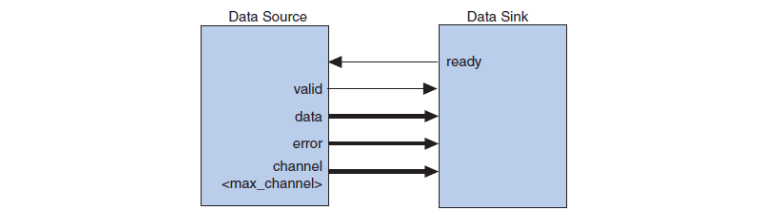
\includegraphics[width=0.8\linewidth]{MasterSlaveST.png}
	\caption{Architecture of the data source and sink.}
	\label{fig:masterslave}
\end{figure}

\noindent Listing \ref{lst:masterslavestsource} shows the application file that takes care of the declaration and wiring of channels, the clock and starting the application.

\begin{lstlisting}[style=customc++, caption=Application file for mater/slave.,
label={lst:masterslavestmain}]
int sc_main(int argc, char* argv[]) {
	
	Source Master("Master"); DataSink Slave("Slave");
	
	sc_clock clock("clock", sc_time(CLK_PERIODE, SC_NS) ); // 50 MHz
	
	sc_signal<bool> ready_channel("C1"), valid_channel("C2") ;
	
	sc_signal<sc_uint<DATA_BITS> >  data_channel("C3");
	sc_signal<sc_uint<ERROR_BITS> > error_channel("C4");
	sc_signal<sc_uint<CHANNEL_BITS> > channel_channel("C5");
	
	Master.valid(valid_channel);
	Master.data(data_channel);
	Master.ready(ready_channel);
	Master.error(error_channel);
	Master.channel(channel_channel);
	Master.clk(clock);
	Slave.valid(valid_channel);
	Slave.data(data_channel);
	Slave.ready(ready_channel);
	Slave.error(error_channel);
	Slave.channel(channel_channel);
	Slave.clk(clock);
	sc_start(2000,SC_NS); return 0; }
\end{lstlisting}
\newpage
\noindent Listing \ref{lst:masterslavestsource} shows the implementation of the source. The outgoing channels are modeled with the \textit{sc\_out} class and ingoing with \textit{sc\_in}. The constructor declares a \textit{source\_method()} sensitive to the  clock configured in the application file. The method detects the ready signal from the sink and then writes a arbitrary number to the data channel, a random error code and a channel bit. Finally it sets the valid channel to true, letting the sink know data is ready.

\begin{lstlisting}[style=customc++, caption=Implementation of the data source.,
label={lst:masterslavestsource}]
SC_MODULE(Source){

	sc_in<bool> ready;
	sc_in_clk clk;

	sc_out<bool> valid;
	sc_out< sc_uint<DATA_BITS> > data;
	sc_out< sc_uint<ERROR_BITS> > error;
	sc_out< sc_uint<CHANNEL_BITS> > channel;

	void source_method(void) {
		if(ready.read() == true){
		data.write(rand() % 65536);
		error.write(rand() % 4);
		channel.write(rand() % MAX_CHANNEL);
		valid.write(true);
	} else {
		valid.write(false);
	}
}

SC_CTOR (Source) {
	SC_METHOD(source_method)
	sensitive << clk;
	dont_initialize();
	}
};
\end{lstlisting}
\newpage
\noindent Listing \ref{lst:masterslavestsink} details the sink. Data is received when valid is signaled, stored and written to an external text file. The global clock invokes the \textit{sink\_method()} method. The text file and the waveform file are opened in the constructor and closed in the destructor. 

\begin{lstlisting}[style=customc++, caption=Implementation of the data sink.,
label={lst:masterslavestsink}]
SC_MODULE(DataSink){

	ofstream myfile;
	
	sc_out<bool> ready;
	sc_in_clk clk;
	
	sc_in<bool> valid;
	sc_in< sc_uint<DATA_BITS> > data;
	sc_in< sc_uint<ERROR_BITS> > error;
	sc_in< sc_uint<CHANNEL_BITS> > channel;

	sc_trace_file * tf;

	void sink_method(void) {
		if(valid.read() == true) {
			int data = this->data.read();
			int error = this->error.read();
			int channel = this->channel.read();

			ready.write(false);

			.. // print data to console and file
		} else {
			ready.write(true);
		}
}

SC_CTOR (DataSink) {
	SC_METHOD(sink_method)
	sensitive << clk;
	dont_initialize();

	...	// code for generating VCD file
	myfile.open ("data.txt");
}

~DataSink() {
	sc_close_vcd_trace_file(tf);
	myfile.close();
	}
};
\end{lstlisting}
\newpage
\noindent Listing \ref{lst:sinkoutput} shows a small snippet from the text file with data entries and figure \ref{fig:gtkwavesignalstate} displays the signal states when the first data transfer occurs from the source at time 10$NS$. It starts when the clock goes low. The data value is 4567, and the valid signal is set accordingly.

\begin{lstlisting}[caption=Output at the sink., frame=single, captionpos=b, label={lst:sinkoutput}]
Data: 17767
Data: 18547
Data: 37962
Data: 31949
Data: 16882
Data: 57670
\end{lstlisting}

\begin{figure}[h]
	\centering
	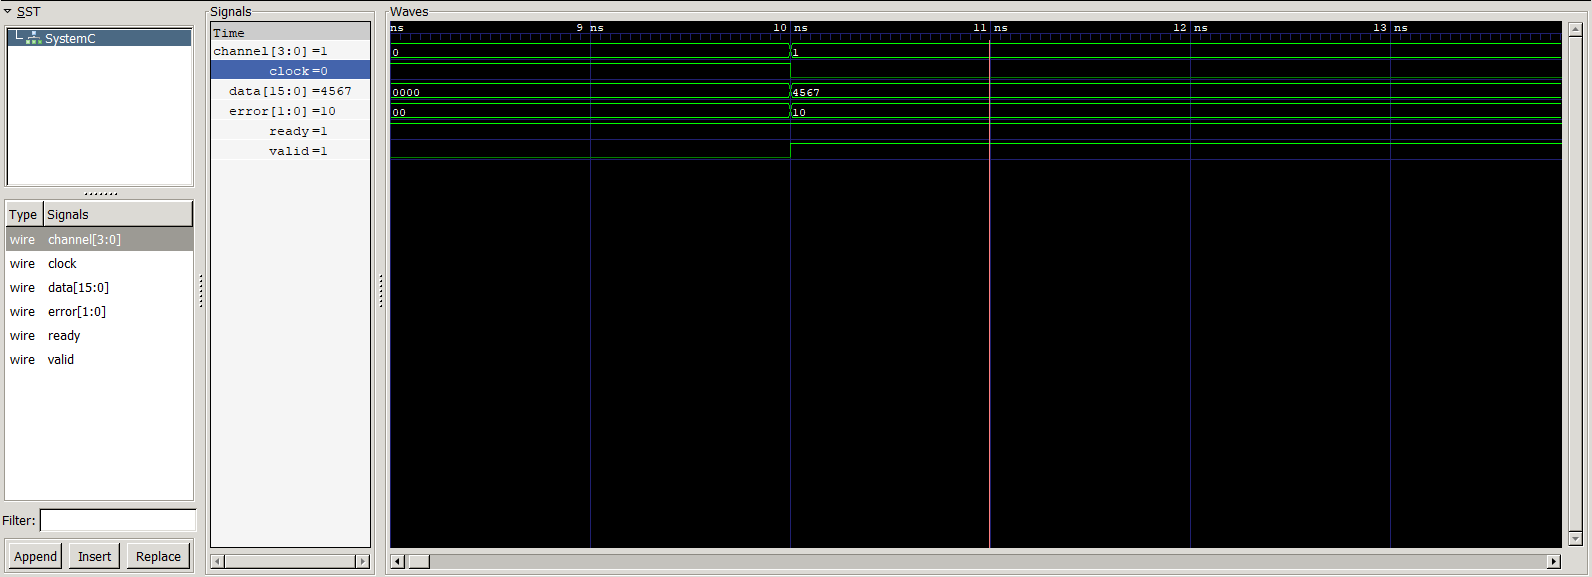
\includegraphics[width=1\linewidth]{MasterSlaveSTGTKWave.png}
	\caption{The signal state monitored in GTKWaveViewer.}
	\label{fig:gtkwavesignalstate}
\end{figure}